
\begin{figure*}
\begin{center}
  % \vspace*{-.55in}
  \hspace*{-.25in}
  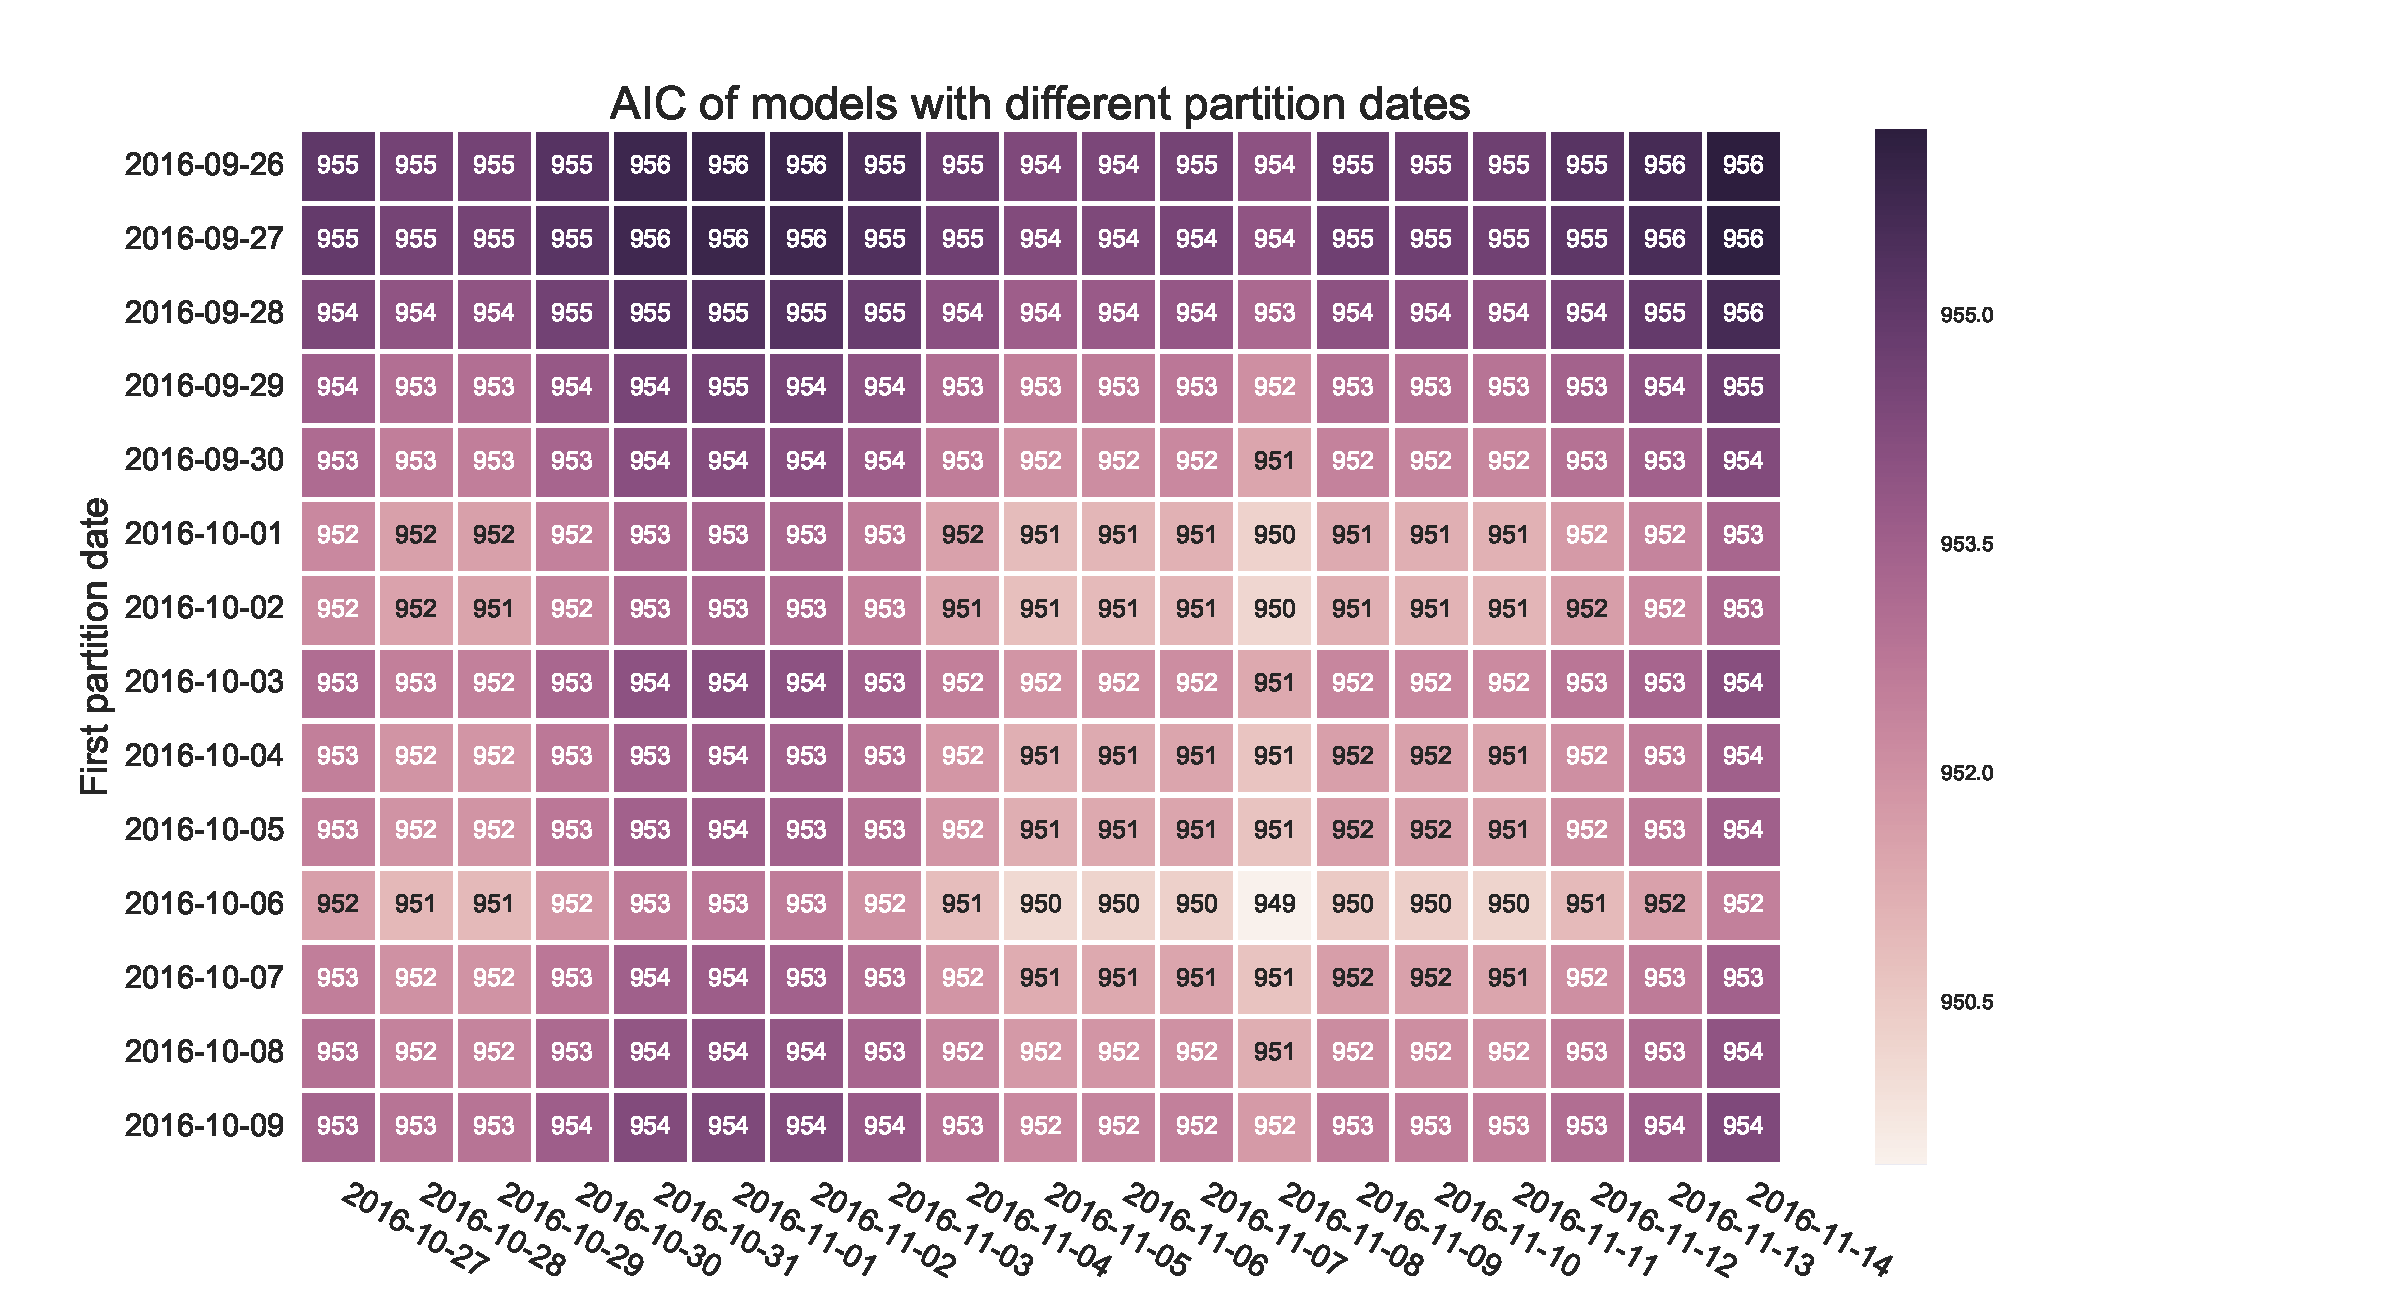
\includegraphics[width=1.25\textwidth]{figures/AIC_dates-FIG2.pdf}
\end{center}
\caption{
  7-day moving average and daily counts of the figurative uses of the three-most
  used violent words in figurative constructions. Uses come from a variety of
  conceptual metaphors which more or less reduce to 
  \textsc{politics is a physical fight}. The first three dashed 
  vertical lines are the dates of the presidential debates, 
  September 26, October 9, and October 19, 2016. The last dashed
  line is election day, November 8, 2016.
}
\label{fig:}
\end{figure*}


\begin{figure*}
\begin{center}
  % \vspace*{-.55in}
  \hspace*{-.25in}
  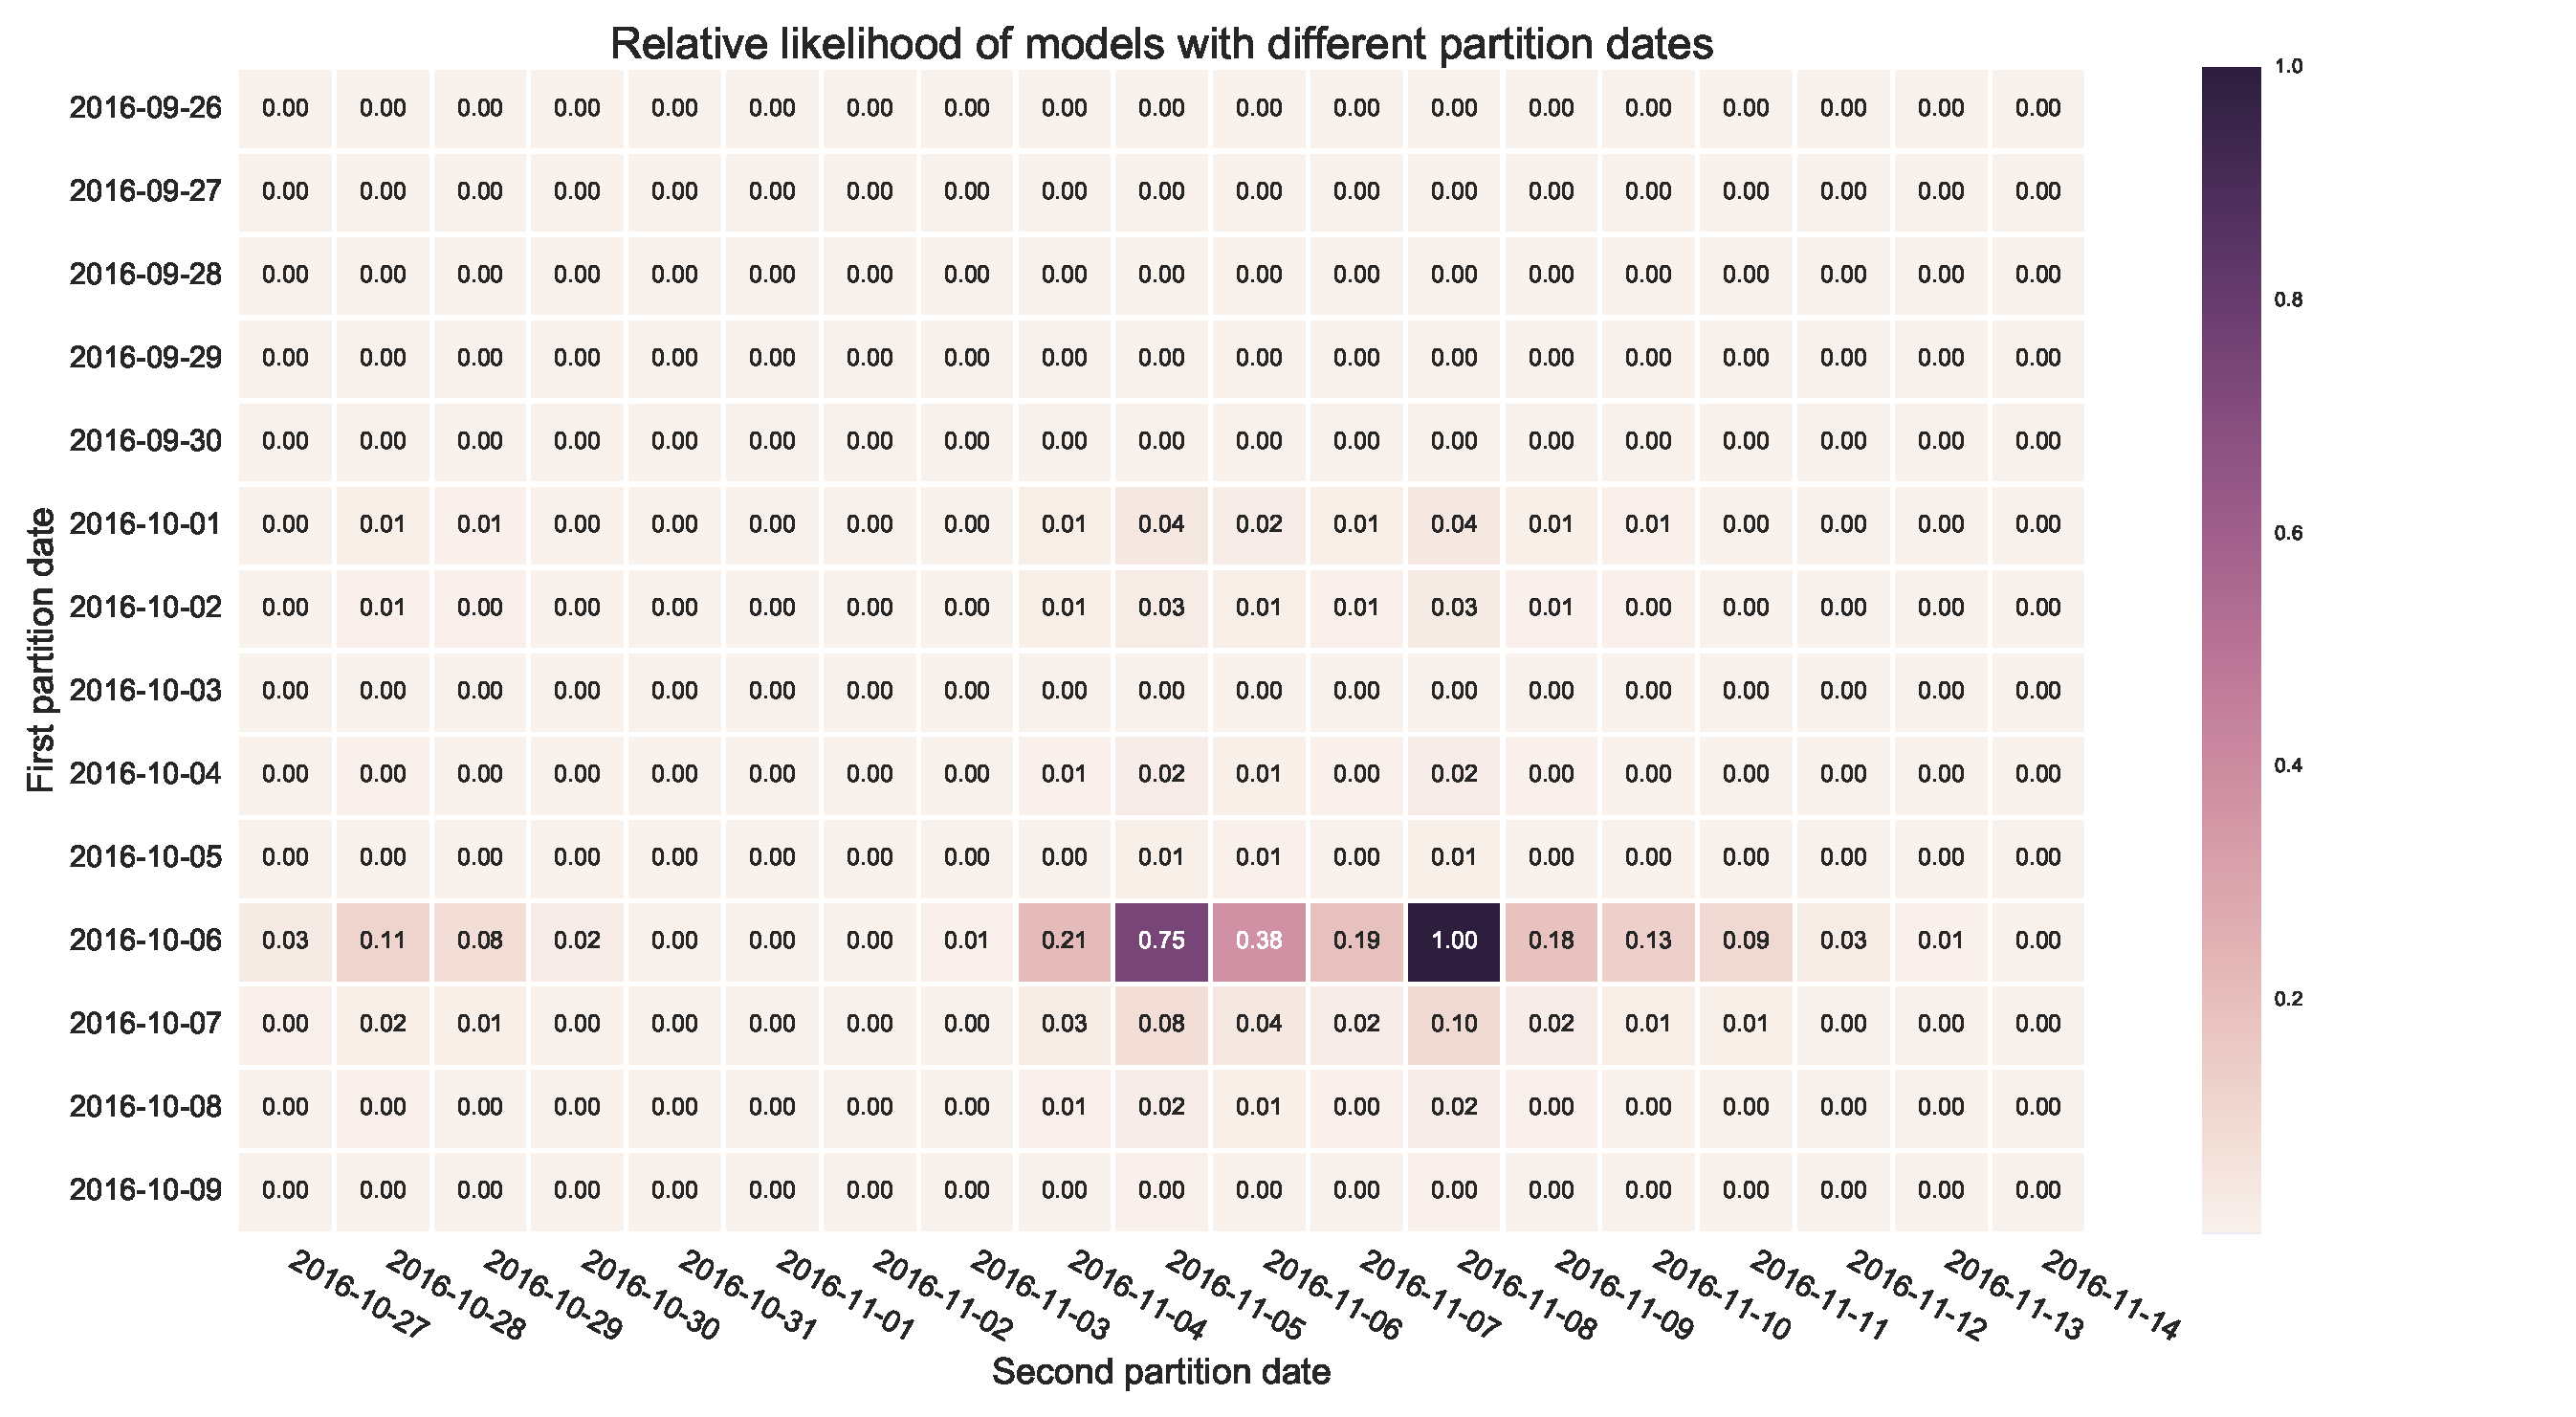
\includegraphics[width=1.25\textwidth]{figures/rel_likelihood_dates-FIG2.pdf}
\end{center}
\caption{
  Relative likelihood of models with identical formula, but different dates
  used to partition the data into three ``phases''. 
}
\label{fig:}
\end{figure*}


% \subsection{Subjects and objects of metaphorical violence}
% \label{sub:Subjects-and-objects-of-metaphorical-violence}

% \newpage

% \begin{figure}
% \begin{center}
%   \includegraphics[width=1.0\textwidth]{figures/trump-clinton-subjects-by-phase.pdf}
% \end{center}
% \caption{Number of times Hillary Clinton and Donald Trump were the subject, or
%   the doer, of the metaphorical violence.}
% \label{fig:trump-clinton-subjects}
% \end{figure}

% \newpage

% \begin{figure}
% \begin{center}
%   \includegraphics[width=1.0\textwidth]{figures/trump-clinton-objects-by-phase.pdf}
% \end{center}
% \caption{Number of times Hillary Clinton and Donald Trump were the object, or
%   the victim, of the metaphorical violence.}
% \label{fig:trump-clinton-objects}
% \end{figure}
